\section{Risultati}
In questa sezione di relazione verranno esposti i risultati restituiti dal HEC-RAS.\\
Grazie alle sezioni di profilo \eqref{figure:profili}, è possibile ricavare il massimo andamento del flusso dell'evento. Inoltre, mediante la funzione simil-gis di RasMapper, è possibile interrogare i singoli layer e ricavare i valori puntuali per ogni punto interno al dominio di calcolo.

\subsection{Flusso transitato nel fiume Boite e Piave}
I diagramma di velocità e profondità del tirante sono riportati successivamente \eqref{figure:depth_boite}\eqref{figure:velocity_boite}\eqref{figure:depth_piave}\eqref{figure:velocity_piave}.\\
I profili utilizzati sono quelli denominati ``profilo\textunderscore boite" e ``profilo\textunderscore piave".

\begin{figure}[htb] \centering
    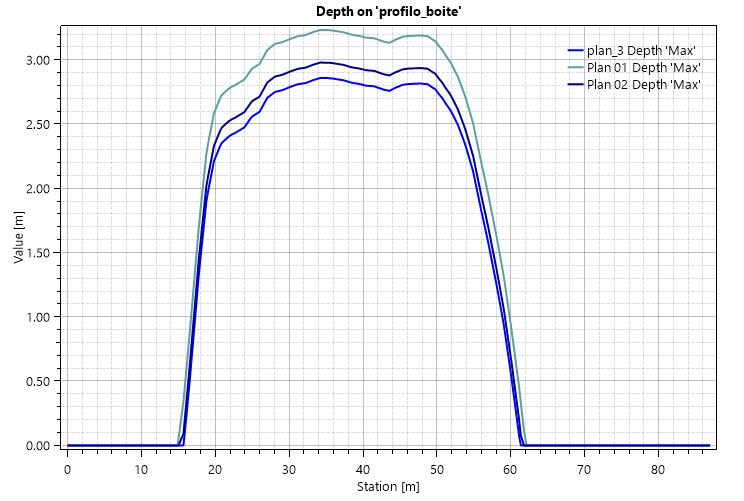
\includegraphics[scale=0.5]{immagini/depth_boite.JPG}
    \caption{Andamento del tirante idraulico, durante l'evento di piena, nel fiume Boite.}
    \label{figure:depth_boite}
\end{figure}

\begin{figure}[htb] \centering
    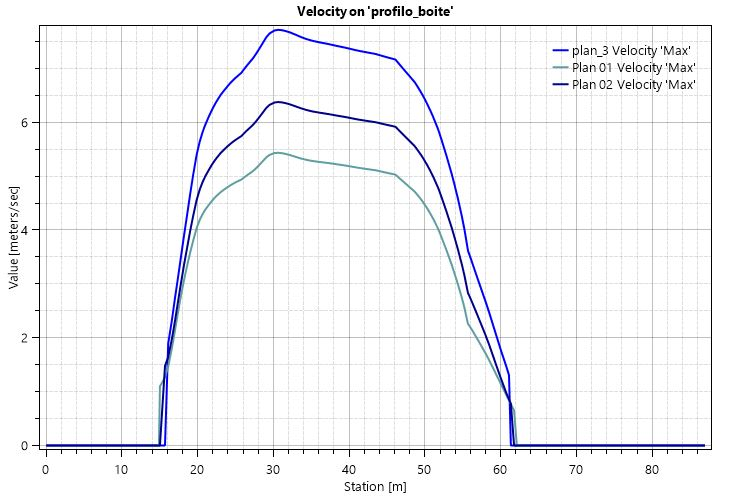
\includegraphics[scale=0.5]{immagini/velocity_boite.JPG}
    \caption{Andamento della velocità di flusso, durante l'evento di piena, nel fiume Boite.}
    \label{figure:velocity_boite}
\end{figure}

\begin{figure}[htb] \centering
    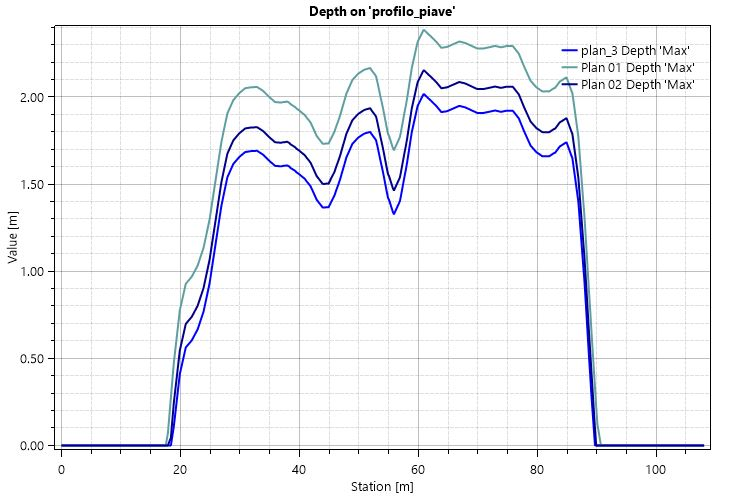
\includegraphics[scale=0.5]{immagini/depth_piave.JPG}
    \caption{Andamento del tirante idraulico, durante l'evento di piena, nel fiume Piave.}
    \label{figure:depth_piave}
\end{figure}

\begin{figure}[htb] \centering
    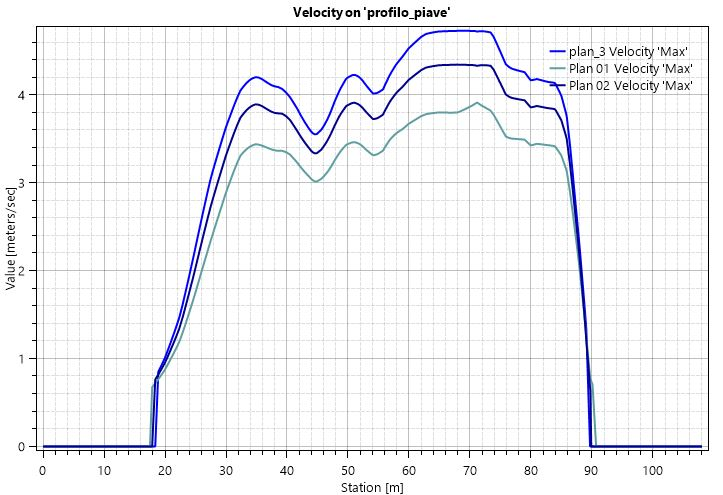
\includegraphics[scale=0.5]{immagini/velocity_piave.JPG}
    \caption{Andamento della velocità di flusso, durante l'evento di piena, nel fiume Piave.}
    \label{figure:velocity_piave}
\end{figure}

E' interessante notare la differenza tra l'andamento della velocità del fiume Piave \eqref{figure:velocity_piave} e del fiume Boite \eqref{figure:velocity_boite}: quest'ultima ha una maggiore omogeneità di valori massimi rispetto alla prima; tale caratteristica potrebbe essere dovuta alla differente geometria del letto dell'alveo.

\subsection{Flusso in uscita dal dominio}
In questa sottosezione verranno esposti i risultati della simulazione nel tratto a valle dell'abitato, in prossimità dell'uscita dal dominio di calcolo.\\
Il profilo da cui sono stati ricavati gli idrogrammi è stato denominato  ``profilo\textunderscore piave\textunderscore outflow".\\
I diagrammi risultanti sono \eqref{figure:depth_piave_outflow}\eqref{figure:velocity_piave_outflow}.

\begin{figure}[htb] \centering
    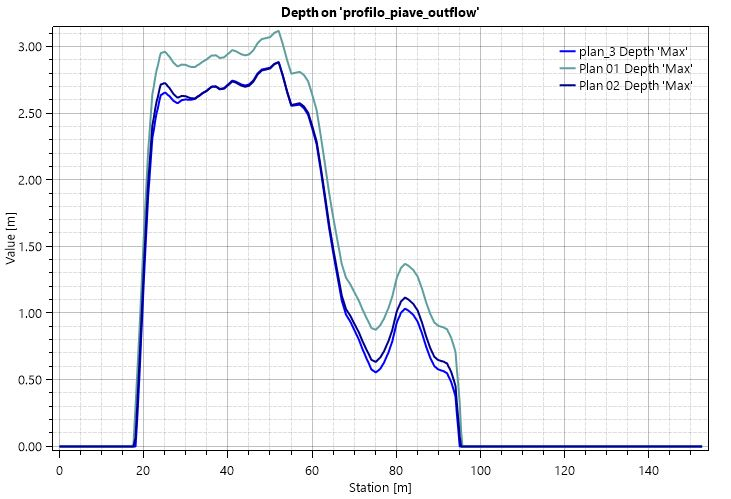
\includegraphics[scale=0.5]{immagini/depth_piave_outflow.JPG}
    \caption{Andamento del tirante idraulico, durante l'evento di piena, nel tratto finale del fiume Piave.}
    \label{figure:depth_piave_outflow}
\end{figure}

\begin{figure}[htb] \centering
    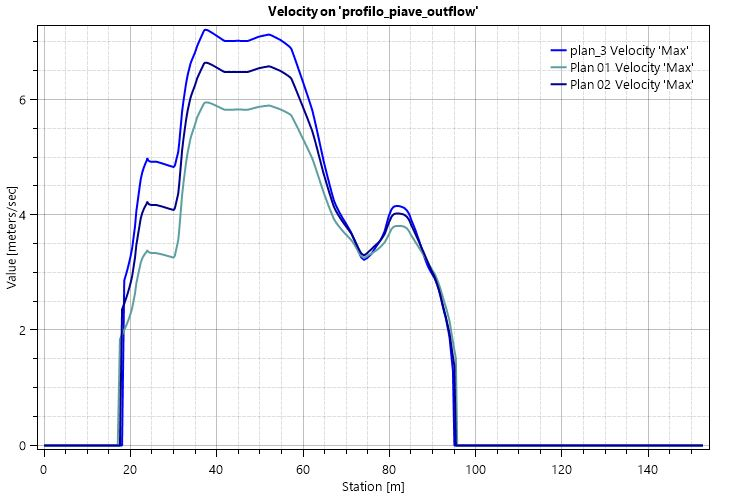
\includegraphics[scale=0.5]{immagini/velocity_piave_outflow.JPG}
    \caption{Andamento della velocità di flusso, durante l'evento di piena, nel tratto finale del fiume Piave.}
    \label{figure:velocity_piave_outflow}
\end{figure}

I risultati sono concordi con quanto previsto: per la simulazione con un Manning relativamente maggiore (ovvero ``plan\textunderscore 1"), la profondità del tirante è maggiore rispetto alle altre due simulazioni. Lo stesso ragionamento può essere fatto con le velocità: il risultato della simulazione con un valore di Manning inferiore agli altri due (ovvero ``plan\textunderscore 3") ha restituito una velocità del flusso ben superiore agli altri due casi.

\subsection{Andamento in prossimità dei ponti}
Lo studio del cinematismo in prossimità del ponte può risultare utile per studiare i possibili casi di rigurgito \cite{rigurgito}.\\
Essendoci due ponti, i profili individuati in alveo sono 4: uno a monte ed uno a valle per ciascuno \eqref{figure:depth_monte_ponte_boite}\eqref{figure:depth_valle_ponte_boite}\eqref{figure:depth_monte_ponte_piave}\eqref{figure:depth_valle_ponte_piave}.

\begin{figure}[htb] \centering
    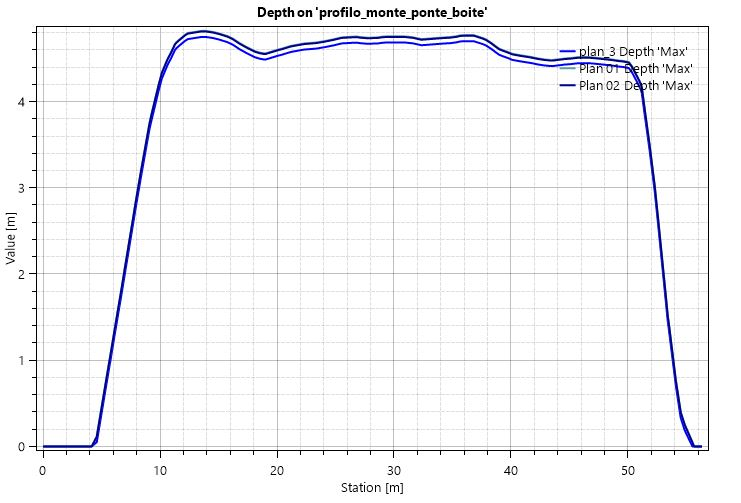
\includegraphics[scale=0.5]{immagini/depth_monte_ponte_boite.JPG}
    \caption{Andamento del tirante idraulico, durante l'evento di piena, a monte del ponte nel fiume Boite.}
    \label{figure:depth_monte_ponte_boite}
\end{figure}

\begin{figure}[htb] \centering
    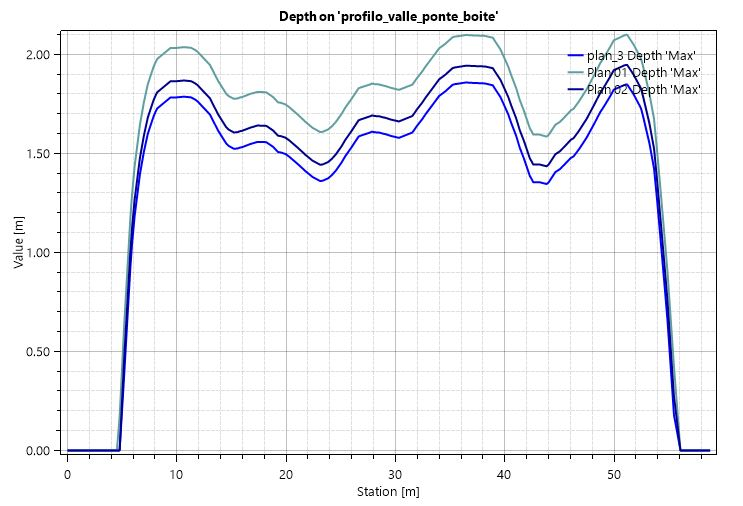
\includegraphics[scale=0.5]{immagini/depth_valle_ponte_boite.JPG}
    \caption{Andamento del tirante idraulico, durante l'evento di piena, a valle del ponte nel fiume Boite.}
    \label{figure:depth_valle_ponte_boite}
\end{figure}

\begin{figure}[htb] \centering
    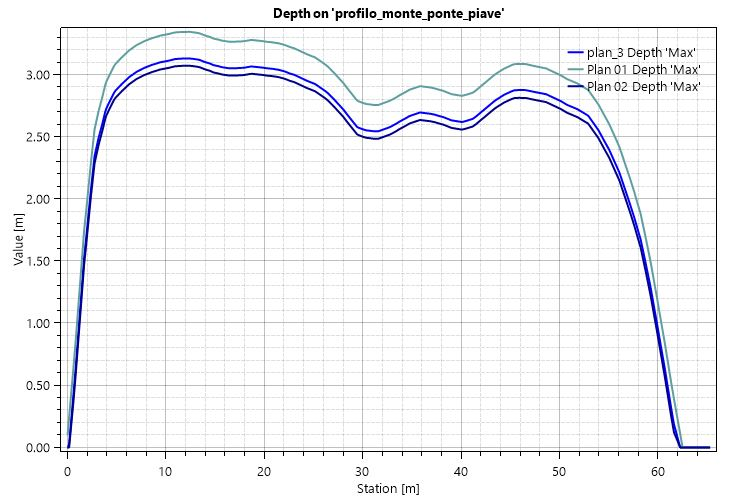
\includegraphics[scale=0.5]{immagini/depth_monte_ponte_piave.JPG}
    \caption{Andamento del tirante idraulico, durante l'evento di piena, a monte del ponte nel fiume Piave.}
    \label{figure:depth_monte_ponte_piave}
\end{figure}

\begin{figure}[htb] \centering
    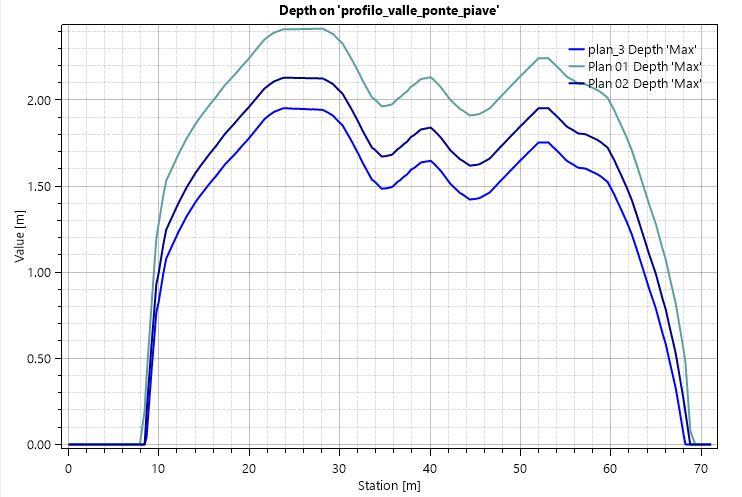
\includegraphics[scale=0.5]{immagini/depth_valle_ponte_piave.JPG}
    \caption{Andamento del tirante idraulico, durante l'evento di piena, a valle del ponte nel fiume Piave.}
    \label{figure:depth_valle_ponte_piave}
\end{figure}

Anche in questo caso, è possibile notare come la profondità del corso d'acqua sia maggiore per l'evento di piena con i valori di Manning maggiori (come per esempio la prima simulazione).

\subsection{Evento di esondazione}
Dai risultati delle simulazioni, risulta semplice notare il verificarsi di una esondazione del fiume nel centro abitato del paese di Perarolo di Cadore.\\
Ai fini di protezione civile, è importante conoscere i volumi esondati ed il tirante d'acqua che si genera nelle aree interessate.
